\chapter{Scepia}\thumbforchapter
\chapterauthor{Rebecca Snabel*, Maarten van der Sande*, Gert Jan Veenstra, Simon J. van Heeringen}
\newpage

\section{Introduction}

\section{Methods}

\subsection{Data collection}

This is from ANANSE:
To generate a collection of putative enhancer regions, we collected all transcription factor ChIP-seq peaks from ReMap 2018 (\href{http://remap.univ-amu.fr/storage/remap2018/hg38/MACS/remap2018_all_macs2_hg38_v1_2.bed.gz}{http://remap.univ-amu.fr/storage/remap2018/hg38/MACS/remap2018\_all\_macs2\_hg38\_v1\_2.bed.gz}) (\href{javascript:;}{41}). We took the summit of all peaks and extended these 25 bp up- and downstream. Based on this file, we generated a coverage bedGraph using bedtools genomecov (\href{javascript:;}{78}). We performed peak calling on this bedGraph file using bdgpeakcall from MACS2 (version v2.7.1) (\href{javascript:;}{69}), with the following settings: \textit{l} = 50 and \textit{g} = 10. We performed the peak calling twice, setting \textit{c} to 4 and 30, respectively. All peaks from \textit{c} = 30 were combined with all peaks of \textit{c} = 4 that did not overlap with the peaks of \textit{c} = 30. We then removed all regions on chrM and extended the summit of the peaks 100 bp up- and downstream to generate a final collection of 1 268 775 putative enhancers of 200 bp. This collection of enhancers is available at Zenodo with doi 10.5281/zenodo.4066423.

Regulatory potential database was made by downloading all human bam files from ENCODE.

Preprocessing of reads was done automatically by seq2science v1.0.3 (https://doi.org/10.5281/zenodo.3921913) using the rna-seq workflow. Public samples were downloaded from the Sequence Read Archive (https://doi.org/10.1093/nar/gkq1019) with help of the ncbi e-utilities and pysradb (https://doi.org/10.12688/f1000research.18676.1). Genome assembly GRCh38.p13 was downloaded with genomepy 0.16.1 (https://doi.org/10.1093/bioinformatics/btad119). Paired-end reads were trimmed with fastp v0.23.2 (https://doi.org/10.1093/bioinformatics/bty560) with default options. Single-end reads were trimmed with fastp v0.23.2 (https://doi.org/10.1093/bioinformatics/bty560) with default options. Reads were aligned with STAR v2.7.10b (https://dx.doi.org/10.1093\%2Fbioinformatics\%2Fbts635) with default options. Afterwards, duplicate reads were marked with Picard MarkDuplicates v3.0.0 (http://broadinstitute.github.io/picard). Bam files were converted to cram format with samtools samtools v1.16 (https://doi.org/10.1093/bioinformatics/btp352). Sample sequencing strandedness was inferred using RSeQC v5.0.1 (https://doi.org/10.1093/bioinformatics/bts356) in order to improve quantification accuracy. Read counting and summarizing to gene-level was performed on filtered bam using HTSeq-count v2.0.2 (https://doi.org/10.1093/bioinformatics/btu638). TPM normalized gene counts were generated using genomepy based on longest transcript lengths.

\subsection{Bulk comparison}

The 

\subsection{Single-cell comparison}


\subsection{Scepia}

\begin{figure}
    \centering
    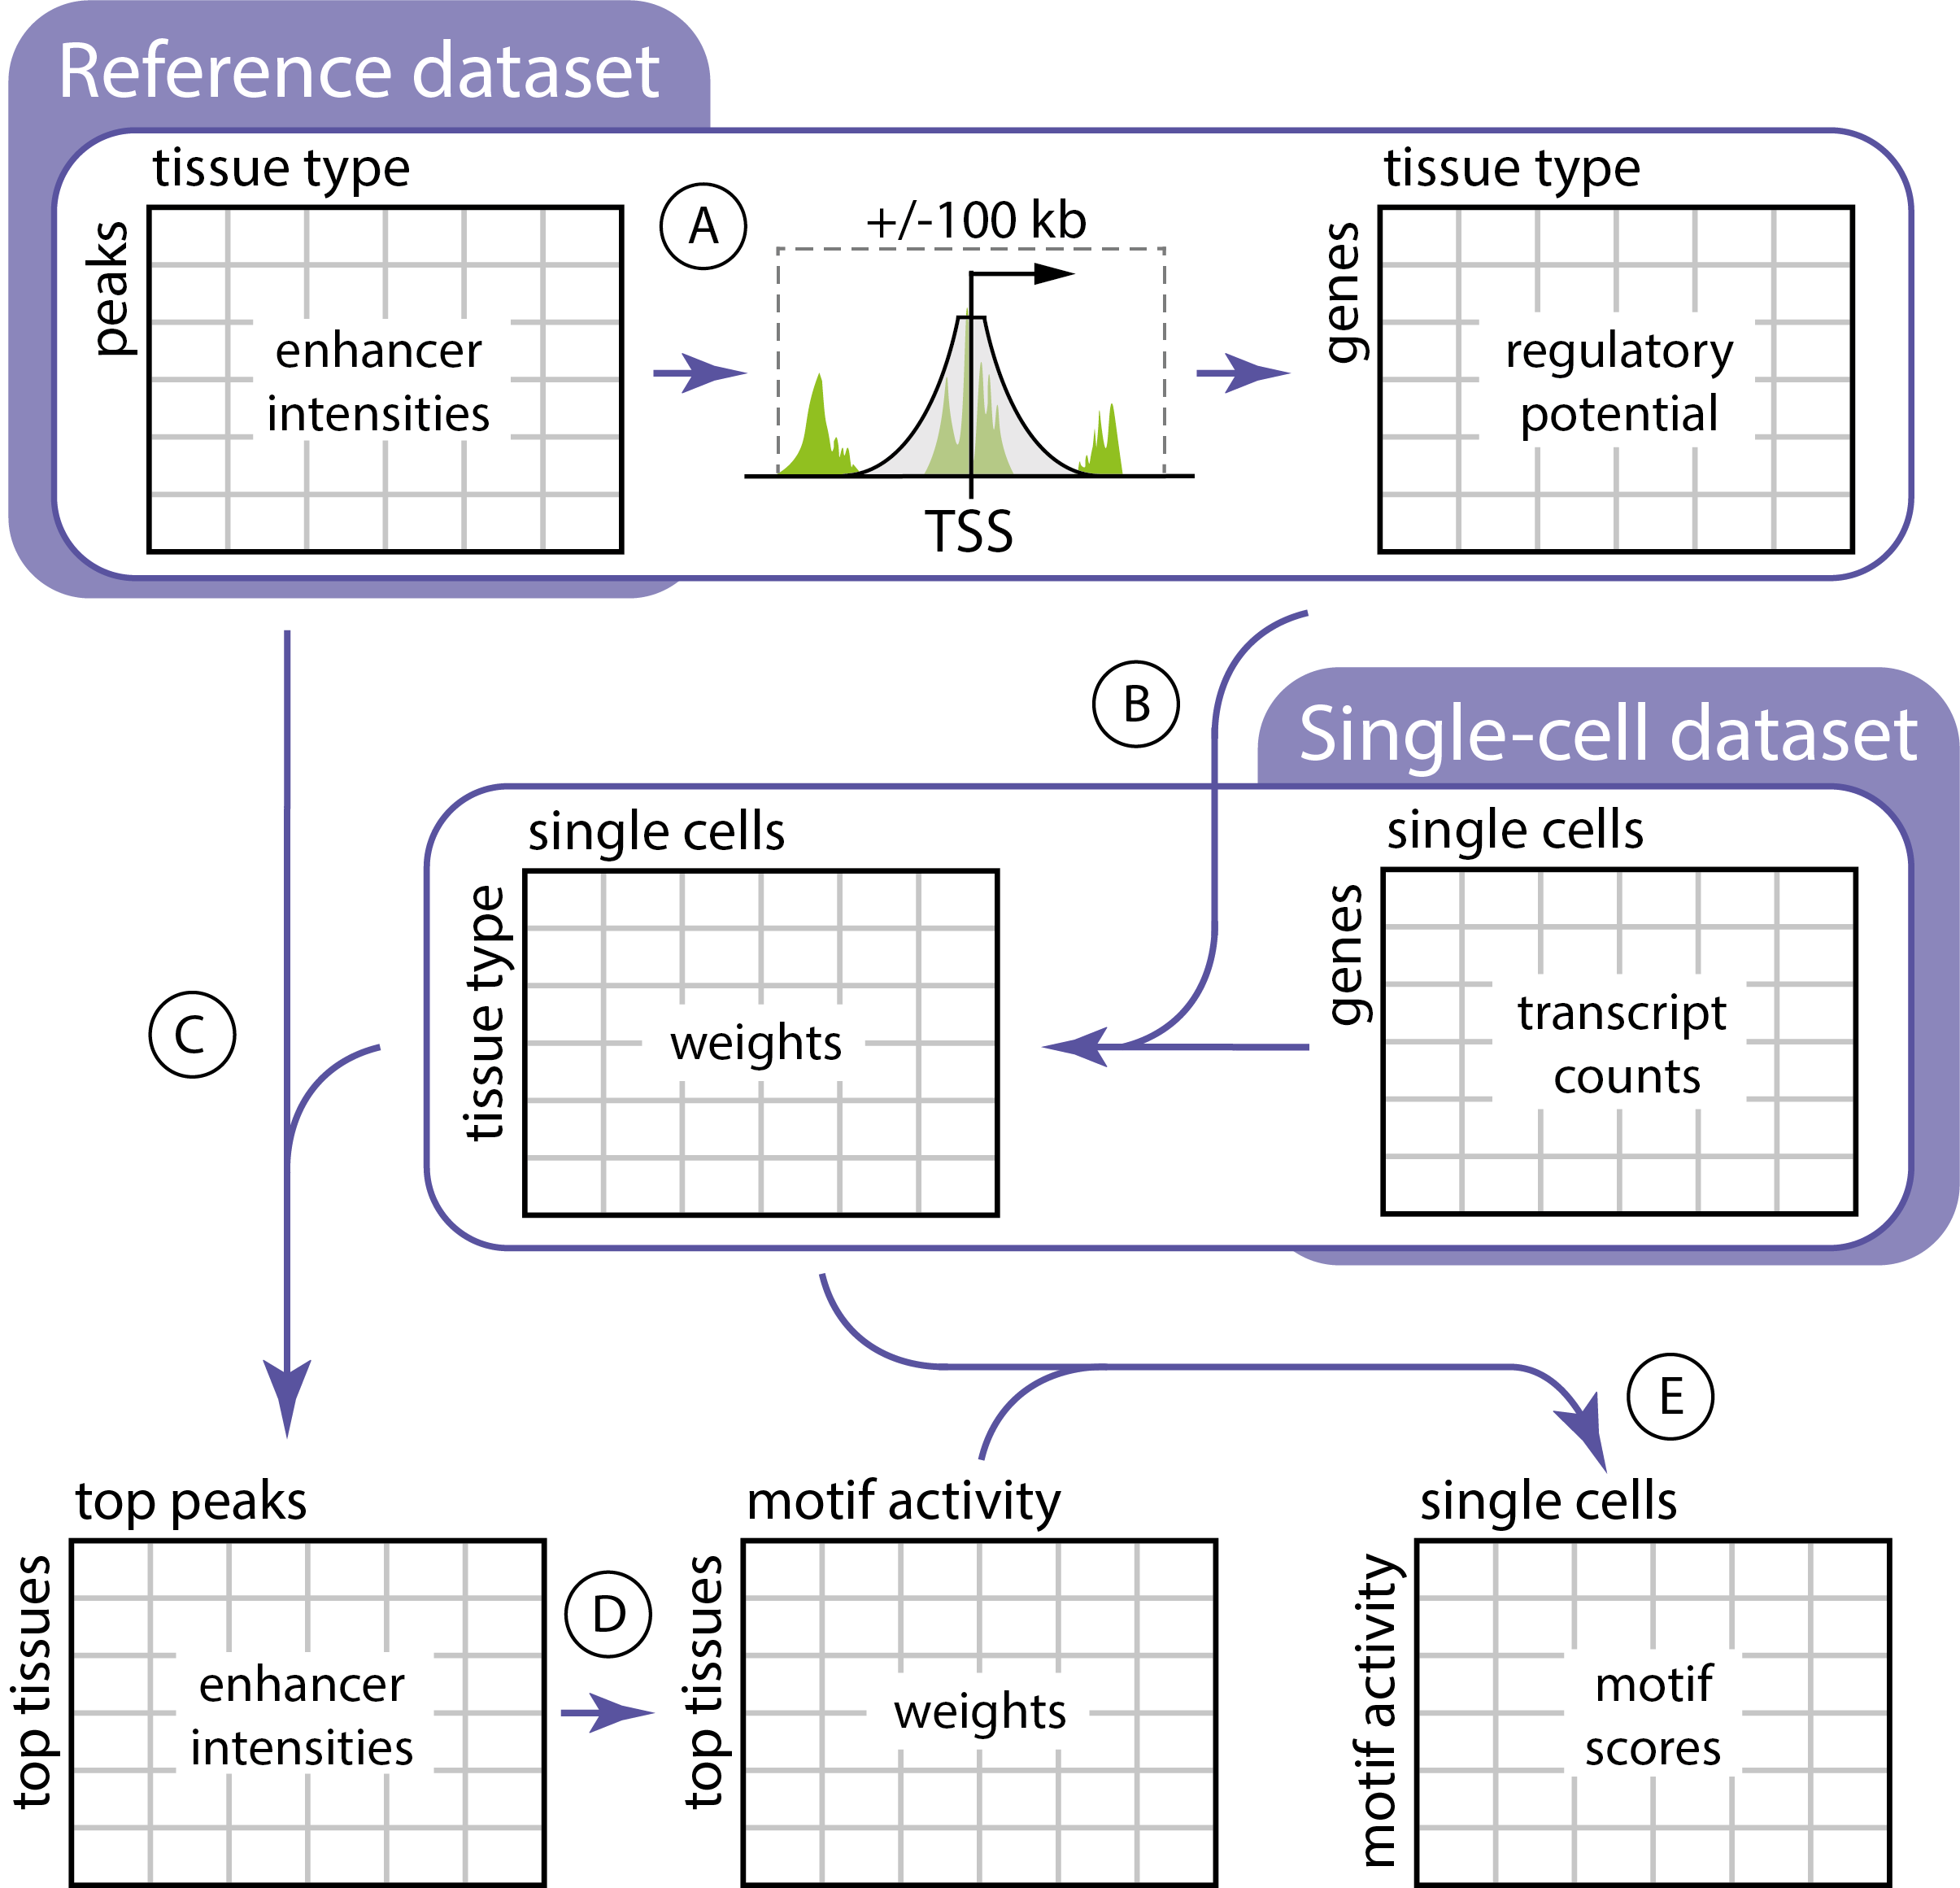
\includegraphics[width=1\linewidth]{ch.scepia/imgs/overview.png}
    \caption{TODO caption}
    \label{fig:enter-label}
\end{figure}

\noindent
Input:

\begin{itemize}
	\item reference Database:
    \begin{itemize}
        \item Let D be the reference database of H3K27ac or other genome-wide measurements related to enhancer "activity". D is represented as a matrix with dimensions (peaks x cell types).
    \end{itemize}
	\item Single-cell dataset:
    \begin{itemize}
        \item Let S be the single-cell dataset. S is represented as a matrix with dimensions (cells x genes).
    \end{itemize}
\end{itemize}

% TODO TISSUE TYPES OR CELL TYPES? Or sth else?

\noindent
This is how scepia works:

\begin{enumerate}[label=(\Alph*)]
    \item Convert the reference database matrix of enhancer intensities (D) into a database matrix of regulatory potential per gene (P).
    \begin{itemize}
        \item Let P be the regulatory potential. P is represented as a matrix with dimensions (genes x cell types)
        \item \begin{equation*}{B_{x,\ r}} = \sum\limits_k {{w_{k,r}}{s_{k,x}}\ } \end{equation*}
        \item Where X , Y , Z etc
        \item \begin{equation*} w_k=\left\{\begin{matrix} 1, && k\epsilon (0\,{\rm kb},\ 5\,{\rm kb}]\\ \frac{2{\rm e}^{-\mu|k-t_r|} }{1+{\rm e}^{-\mu|k-t_r|}}, && k\epsilon (5\,{\rm kb},\ 100\,{\rm kb}] \end{matrix}\right. \end{equation*}
        \item Where X , Y , Z etc
    \end{itemize}
    \item Weigh each cell in the single-cell dataset (S) with regulatory potential (P) resulting in annotation matrix A.
    \begin{itemize}
        \item Let A be the cell type Annotation matrix. A is represented as a matrix with dimensions (cells x cell types)
        \item We do a lasso regression to infer the annotation weights: $S_i = P_i A_i + \lambda ||A_i||_1 +\epsilon$
        \item this is much more complex, as we first take cluster most common, then do it for each cell based on average neighbour gene expression, and finally, take the average cell type annotation of the neighbours..
    \end{itemize}
    \item Take the cell type annotations, and find the top most differential enhancers.
    \begin{itemize}
        \item $E_i = argmax_j(A_i)$
    \end{itemize}
    \item Do a motif scan
    \begin{itemize}
        \item matrix M
        \item We do a bayesian ridge regression to infer the motif weights TODO formula: $S_i = P_i A_i + \lambda ||A_i||_2^2 +\epsilon$
        \item TODO ridge is $ \underset{\beta}{\operatorname{arg\,min}}\; \|y - X\beta\|^2_2 + \lambda \|\beta\|^2_2 $
    \end{itemize}
    \item dot product of annotation weights and motif scores F
    \begin{itemize}
        \item $F = S \cdot A$
    \end{itemize}
\end{enumerate}

\section{Results}

\subsection{Matching regulatory potential and RNA}

T
\begin{figure}
    \centering
    \includegraphics[width=0.75\linewidth]{ch.scepia/imgs/celltypes.png}
    \caption{Ill encircle some stuff for convincing. Not sure which cmap, all are ugly.. or not colorblind, or red green and thats confusing microarray. Also Ill remove labels in the end?}
    \label{fig:enter-label}
\end{figure}
Since a gene's transcript counts and its regulatory potential are correlated, 
\begin{figure}
    \centering
    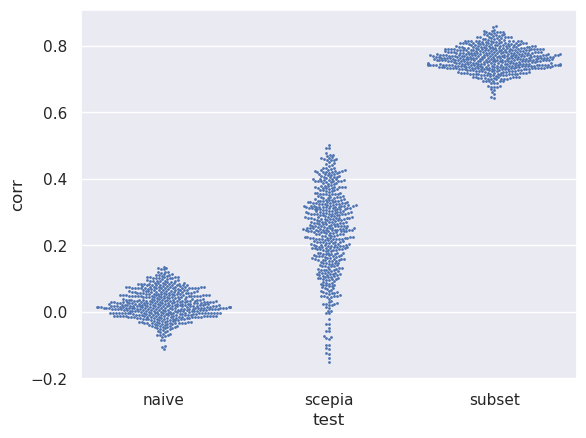
\includegraphics[width=0.75\linewidth]{ch.scepia/imgs/scepia_bulk_benchmark.png}
    \caption{}
    \label{fig:enter-label}
\end{figure}
See supplemental figure XXX for parameter sweep. This is nice because test/validate separate

\subsection{Single-Cell Epigenome-based Inference of Activity}

\section{Discussion}

\subsection{Limitations}
\begin{itemize}
    \item Benchmark is bad. Benchmarking against a bad ground truth is stupid.
    \item 
\end{itemize}

\section{Supplementals}
\beginsupplement
\begin{table}
\begin{center}
\begin{tabular}{||c c c c||} 
\hline
Weight curve & Correlation between & Correct specific & Correct broad \\[0.5ex] 
\hline
Ananse & $0.53 \pm 0.14$ & $64\%$ & $77\%$ \\ 
\hline
Wang & $0.54 \pm 0.15 $ & $64\%$ & $75\%$ \\
\hline
Promoter (5kb) & $0.54 \pm 0.14$ & $66\%$ & $77\%$ \\
\hline
Enhancer & $0.43 \pm 0.14$ & $60\%$ & $72\%$ \\
\hline
\end{tabular}
\caption{Caption of my table.}
\label{table:1}
\end{center}
\end{table}
